\documentclass[10pt, conference, compsocconf]{IEEEtran}

%\usepackage{cite}
\usepackage[utf8]{inputenc}
\usepackage{graphicx}
\usepackage{epstopdf}
\usepackage{amsmath}
\usepackage{multirow}
\usepackage{lipsum}
\usepackage{caption}
\usepackage{subcaption}
\usepackage{setspace}
\usepackage{float}

\renewcommand{\tablename}{Tabela}
\renewcommand{\figurename}{Figura}
\renewcommand{\refname}{Referências}

\begin{document}
\title{Estudo de dados de patologias cardíacas pediátricas}

\author{\IEEEauthorblockN{Filipe Figueiredo}
  \IEEEauthorblockA{201203559}
  \and
  \IEEEauthorblockN{Pedro Paredes}
  \IEEEauthorblockA{201205725}
}

\newcommand{\PreImg}[1]{
  \begin{figure}[H]
    \centering
    \includegraphics[scale=0.4]{img/pre_#1.png}
    \caption{Distribuição de {\tt #1} em relação a {\tt nxa}}
    \label{fig:pre#1}
  \end{figure}
}

\maketitle

% ----------------------------------------
% -                                      -
% ----------------------------------------

\section{Introdução}
\label{sec:int}

O uso de métodos estatísticos e computacionais para o estudo de dados
reais. Graças à evolução de métodos avançados de previsão e regressão,
uma área conhecida por ``Aprendizagem de Máquina'' (ou \textit{Machine
  Learning}), é possível estudar diversos problemas em diferentes
contextos. Esta análise é normalmente precedida de uma vasta análise
exploratória dos dados com diferentes fins, como a seleção de
atributos chave (por exemplo, através da determinação da correlações
entre os vários atributos) ou como a eliminação de \textit{outliers}
estatísticos.

Neste trabalho, aplicamos várias destas técnicas comuns a um conjunto
de dados de patologias cardíacas de casos pediátricos. O objetivo
final é determinar quais variáveis têm maior ``poder'' de previsão
para determinar se um determinado sujeito possui alguma anormalidade
cardíaca e estudar o seu erro de classificação.

O resto deste relatório está organizado da seguinte forma. Na
Secção~\ref{sec:apr} descreve-se o \textit{dataset} usado assim como
os seus atributos e propriedades extrínsecas. Segue-se a descrição do
preprocessamento dos dados na Secção~\ref{sec:pre}, onde se indica as
correções base efetuadas por cada atributo e a devida
justificação. Posteriormente, na Secção~\ref{sec:ads} é feita uma
análise descritiva dos dados já processados, com o objetivo de se
estabelecer um perfil base dos dados. Na Secção~\ref{sec:afn} é feita
a análise final dos dados já processados, começando por verificar as
relações entre os pares de atributos e entre múltiplos atributos com
objetivo de efetuar uma escolha informada de atributos a usar para
aplicar algoritmos de classificação para determinar a presença de
anomalias cardíacas. Finalmente, na Secção~\ref{sec:cnd} são feitas
algumas notas finais e uma breve discussão das conclusões obtidas no
corpo do relatório.

% ----------------------------------------
% -                                      -
% ----------------------------------------

\section{Análise preliminar}
\label{sec:apr}

O \textit{dataset} fornecido para análise foi colecionado no Real
Hospital Português do Brasil, tendo sido posteriormente anonimizado e
enviado para Portugal com a autorização do Comité de ética do próprio
hospital. Os dados consistem em crianças entre os 0 e 19 anos, que
possuem ou não patologias cardíacas.

Na lista seguinte descrevemos em detalhe cada atributo presente nos
dados. A sigla de três letras indica o nome usado na análise dos dados
(presente na implementação que será descrita ao longo do relatório).

\begin{description}
  \item[\texttt{id}] Dado categórico que representa o número de identificação
    anonimizado do paciente
  \item[\texttt{pso}] Dado numérico contínuo que representa o peso do
    paciente em quilogramas
  \item[\texttt{alt}] Dado numérico contínuo que representa a altura
    do paciente em centímetros
  \item[\texttt{imc}] Dado numérico contínuo que representa o índice
    de massa corporal do paciente
  \item[\texttt{sex}] Dado categórico que representa o sexo do
    paciente
  \item[\texttt{atd}] Dado numérico discreto que representa a data em
    que o paciente foi atendido (e que os dados deste paciente foram
    colecionados)
  \item[\texttt{dn}] Dado numérico discreto que representa a data em
    que o paciente nasceu
  \item[\texttt{ide}] Dado numérico contínuo que representa a idade do
    paciente em anos
  \item[\texttt{cnv}] Dado categórico que representa a instituição de
    seguro de saúde a que pertence o paciente
  \item[\texttt{pls}] Dado categórico que representa o tipo de pulsos
    do paciente
  \item[\texttt{pas}] Dado numérico discreto que representa a pressão
    sistólica arterial do sangue do paciente em milímetros de mercúrio
  \item[\texttt{pad}] Dado numérico discreto que representa a pressão
    diastólica arterial do sangue do paciente em milímetros de mercúrio
  \item[\texttt{ppa}] Dado categórico que representa a relação entre a
    pressão sistólica e a diastólica do paciente
  \item[\texttt{b2}] Dado categórico que representa o segundo som
    cardíaco (ou o $S_2$) do paciente
  \item[\texttt{spr}] Dado categórico que representa o som cardíaco
    (sopro) do paciente
  \item[\texttt{fc}] Dado numérico discreto que representa a
    frequência de batimentos cardíacos do paciente
  \item[\texttt{hd1}] Dado categórico que representa o historial
    principal de doenças do paciente
  \item[\texttt{hd2}] Dado categórico que representa o historial
    secundário de doenças do paciente
  \item[\texttt{mo1}] Dado categórico que representa o motivo
    principal para admissão clínica do paciente
  \item[\texttt{mo2}] Dado categórico que representa o motivo
    secundário para admissão clínica do paciente
  \item[\texttt{nxa}] Dado categórico que representa a presença ou
    ausência de patologias cardíacas do paciente (atributo a prever)
\end{description}

Antes de se efetuar alguma análise aos dados, foi feita uma limpeza
simples dos dados. Primeiramente removemos as colunas de {\tt id} e
{\tt cnv}, pois são apenas administrativas e não serão úteis para
nenhuma análise. Além disso, renomeamos os atributos para as siglas de
3 letras usadas na descrição anterior, assim como os próprios valores
(por exemplo, no caso da variável {\tt nxa}, todas as entradas
passaram a ser do tipo ``nor'' ou ``ano'', representando
respetivamente, ``normal'' ou ausência de patologia e ``anormal'' ou
presença de patologia). Finalmente foram tirados todos os valores
claramente incorretos, como idades negativas ou acima dos 20 anos,
datas posteriores à data atual \ldots

Tendo estas correções, passaremos a descrever cada atributo que se
manteve. Primeiramente, mostramos um sumário dos atributos numéricos
na Tabela~\ref{tab:nua}

\begin{table*}[!ht] \centering 
  \caption{Sumário dos atributos numéricos}
  \label{tab:nua} 
  \begin{tabular}{@{\extracolsep{5pt}}lccccccc} 
    \\[-1.8ex]\hline 
    \hline \\[-1.8ex] 
    Estatística & {\tt pso} & {\tt alt} & {\tt imc} & {\tt ide} & {\tt pas} & {\tt pad} & {\tt fc} \\ 
    \hline \\[-1.8ex] 
    N & 14,945 & 13,413 & 13,032 & 16,175 & 10,143 & 10,133 & 15,832 \\ 
    Média & 24.9 & 111.8 & 18.0 & 6.3 & 101.3 & 62.3 & 93.8 \\ 
    Desvio Padrão & 17.1 & 33.9 & 12.0 & 4.7 & 15.5 & 8.9 & 100.4 \\ 
    Mínimo & 0.3 & 10 & 5 & 0 & 10 & 6 & 8 \\ 
    Máximo & 157 & 198 & 848 & 19.8 & 990 & 120 & 9,288 \\ 
    {\tt NA}s & 2,928 & 4,460 & 4,841 & 1,698 & 7,730 & 7,740 & 2,041\\
    \hline \\[-1.8ex] 
  \end{tabular}
\end{table*}

Nas seguintes subseções iremos descrever cada um destes atributos em
detalhe, indicando a sua distribuição em relação a {\tt nxa} seguido
de uma breve discussão.

\subsection{\texttt{pso}}
Na Figura~\ref{fig:prepso} está representada a distribuição de valores
do atributo {\tt pso} em relação a {\tt nxa}.

\PreImg{pso}

A distribuição é influenciada pela variação de idades dos pacientes
considerados nos dados. Por esta razão, os dados aparentam ser
bimodais.

\subsection{\texttt{alt}}
Na Figura~\ref{fig:prealt} está representada a distribuição de valores
do atributo {\tt alt} em relação a {\tt nxa}.

\PreImg{alt}

A distribuição é semelhante à distribuição de {\tt pso} (com uma
escala diferente), o que já indica a possibilidade de uma correlação
entre os dois atributos. Adicionalmente, é também fortemente
influenciada pela idade.

\subsection{\texttt{imc}}
Na Figura~\ref{fig:preimc} está representada a distribuição de valores
do atributo {\tt imc} em relação a {\tt nxa}.

\PreImg{imc}

Este atributo é determinado unicamente a partir de {\tt pso} e {\tt
  alt}, o que é mostrado na sua distribuição. Porém, a influência da
idade é diminuída neste caso por ser a razão entre dois atributos com
influência semelhante.

\subsection{\texttt{sex}}
Na Figura~\ref{fig:presex} está representada a distribuição de valores
do atributo {\tt sex} em relação a {\tt nxa}.

\PreImg{sex}

Há uma ligeira tendência para elementos do sexo masculino, mas em
proporção aproximadamente equilibrada (cerca de $35\%$ para
$65\%$). Também é possível observar que a distribuição de {\tt nxa} em
cada um dos sexos é aproximadamente igual à distribuição marginal de
{\tt nxa}. Por isso este atributo não será um bom descritor da
variável {\tt nxa}, o que nos indica que a incidência de anomalias
cardíacas em casos pediátricos é aproximadamente agnóstico em relação
ao sexo.

\subsection{\texttt{atd}}
Na Figura~\ref{fig:preatd} está representada a distribuição de valores
da variável {\tt atd}.

\begin{figure}[H]
  \centering
  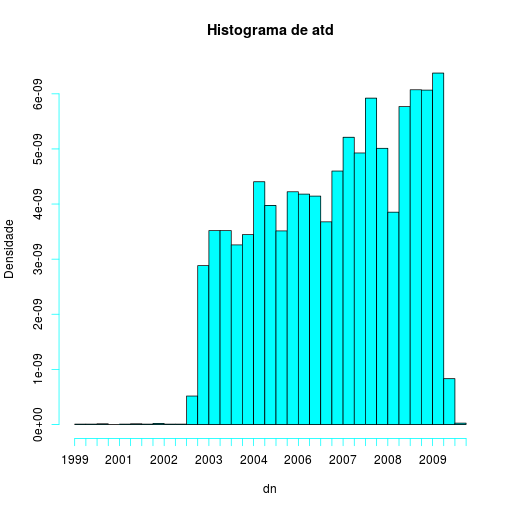
\includegraphics[scale=0.4]{img/pre_atd.png}
  \caption{Distribuição de {\tt atd}}
  \label{fig:preatd}
\end{figure}

\subsection{\texttt{dn}}
Na Figura~\ref{fig:predn} está representada a distribuição de valores
do atributo {\tt dn}.

\begin{figure}[H]
  \centering
  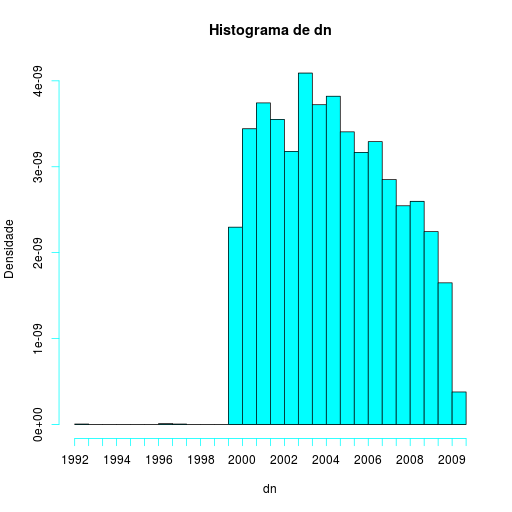
\includegraphics[scale=0.4]{img/pre_dn.png}
  \caption{Distribuição de {\tt dn}}
  \label{fig:predn}
\end{figure}

\subsection{\texttt{ide}}
Na Figura~\ref{fig:preide} está representada a distribuição de valores
do atributo {\tt ide} em relação a {\tt nxa}.

\PreImg{ide}

A distribuição é relativamente equilibrada para {\tt nxa} exceto um
pico para as idades mais baixas que têm uma predominância de
indivíduos com anormalidades cardíacas. Este valor curioso pode ser
explicado pelo facto que uma grande parte das anormalidades cardíacas
ou é genética ou é derivada de complicações do nascimento, sendo por
isso detetadas cedo.

\subsection{\texttt{pls}}
Na Figura~\ref{fig:prepls} está representada a distribuição de valores
do atributo {\tt pls} em relação a {\tt nxa}.

\PreImg{pls}

A maior parte dos pacientes têm pulsos normais, porém, para os que não
têm o valor de {\tt nxa} está muito bem definido. Assim, este atributo
poderá ser um bom descritor de {\tt nxa}.

\subsection{\texttt{pas}}
Na Figura~\ref{fig:prepas} está representada a distribuição de valores
da variável {\tt pas} em relação à {\tt nxa}.

\PreImg{pas}

Os picos na distribuição são devidos ao facto de que nos dados
fornecidos os valores de {\tt pas} serem inteiros (e por isso
provavelmente arredondados).

\subsection{\texttt{pad}}
Na Figura~\ref{fig:prepad} está representada a distribuição de valores
da variável {\tt pad} em relação à {\tt nxa}.

\PreImg{pad}

A distribuição é muito semelhante à de {\tt pas}, indicando uma forte
correlação entre as duas. A presença de picos pode ser explicada da
mesma forma de para {\tt pas}. Ainda assim, é possível observar uma
semelhança a uma distribuição normal unimodal tanto na distribuição de
{\tt pad} como de {\tt pas}.

\subsection{\texttt{ppa}}
Na Figura~\ref{fig:preppa} está representada a distribuição de valores
do atributo {\tt ppa} em relação a {\tt nxa}.

\PreImg{ppa}

A distribuição de {\tt nxa} para cada valor possível deste atributo é
aproximadamente igual à distribuição marginal de {\tt nxa}, que nos
indica que este não será um bom indicador de {\tt nxa}. Pelo facto que
este atributo é totalmente definido por {\tt pas} e {\tt pad}, este
atributo não adiciona muita informação aos dados e por isso será
removido das análises seguintes.

\subsection{\texttt{b2}}
Na Figura~\ref{fig:preb2} está representada a distribuição de valores
do atributo {\tt b2} em relação a {\tt nxa}.

\PreImg{b2}

A maior parte dos indivíduos têm {\tt b2} normal, mas os restantes têm
uma predominância de anomalia cardíacas. Por esta razão, este atributo
será um bom descritor de {\tt nxa} para certos casos.

\subsection{\texttt{spr}}
Na Figura~\ref{fig:prespr} está representada a distribuição de valores
do atributo {\tt spr} em relação a {\tt nxa}.

\PreImg{spr}

A distribuição de {\tt spr} é uma boa indicadora de {\tt nxa}
(aparenta ter uma correlação alta) pois há uma clara divisão de
elementos de {\tt spr} onde predomina uma classe de {\tt nxa}.

\subsection{\texttt{fc}}
Na Figura~\ref{fig:prefc} está representada a distribuição de valores
da variável {\tt fc} em relação à {\tt nxa}.

\PreImg{fc}

Para a frequência cardíaca, certos valores estavam expressos em
intervalo, para estes foi assumido a média dos dois como o valor
real. Pelas mesmas razões que em {\tt pas} e {\tt pad}, existem picos
na distribuição, mas é possível observar uma semelhança a um
distribuição normal unimodal.

\subsection{\texttt{hd1}}
Na Figura~\ref{fig:prehd1} está representada a distribuição de valores
da variável {\tt hd1} em relação à {\tt nxa}.

\PreImg{hd1}

A distribuição de {\tt hd1} parece manter a distribuição marginal de
{\tt nxa} e é não será por isso um bom descritor de {\tt nxa}.

\subsection{\texttt{hd2}}
Na Figura~\ref{fig:prehd2} está representada a distribuição de valores
da variável {\tt hd2} em relação à {\tt nxa}.

\PreImg{hd2}

A distribuição de {\tt hd2} apresenta um número elevado de {\tt NA}s e
por isso este atributo foi removido para as análises futuras.

\subsection{\texttt{mo1}}
Na Figura~\ref{fig:premo1} está representada a distribuição de valores
da variável {\tt mo1} em relação à {\tt nxa}.

\PreImg{mo1}

A distribuição de {\tt mo1} parece manter a distribuição marginal de
{\tt nxa} e é não será por isso um bom descritor de {\tt nxa}.

\subsection{\texttt{mo2}}
Na Figura~\ref{fig:premo2} está representada a distribuição de valores
da variável {\tt mo2} em relação à {\tt nxa}.

\PreImg{mo2}

A distribuição de {\tt mo2} apresenta um número elevado de {\tt NA}s e
por isso este atributo foi removido para as análises futuras.

\subsection{\texttt{nxa}}
Na Figura~\ref{fig:prenxa} está representada a distribuição de valores
da variável {\tt nxa}.

\begin{figure}[H]
  \centering
  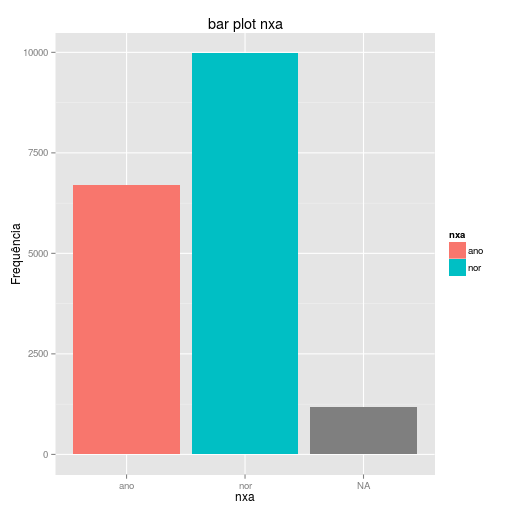
\includegraphics[scale=0.4]{img/pre_nxa.png}
  \caption{Distribuição de {\tt nxa}}
  \label{fig:prenxa}
\end{figure}

Existem alguns valores em falta neste atributo. Como este atributo é o
\textit{label} dos dados, os pacientes sem este valor não são
relevantes para a análise e por isso foram removidos para análise
futura.

% ----------------------------------------
% -                                      -
% ----------------------------------------

\section{Preprocessamento de dados}
\label{sec:pre}

Para preprocessar os dados, começamos primeiramente por verificar a
consistência dos dados. Primeiro comparámos a idade com as datas de
nascimento e atendimento para garantir que os valores eram
consistentes. Depois disto os atributos das datas foram retirados por
já não serem necessários. De seguida removeram-se valores
inconsistentes com o atributo, por exemplo valores de {\tt \#!VALUE}
causados por erros de \textit{software} e do formato de armazenamento
dos dados. De modo a remover entradas pouco descritivas, foram
removidos elementos com mais de $50\%$ de valores em falta. Finalmente
foram removidos entradas em duplicado dos dados.

Nas duas próximas subsecções descrevemos as transformações de dados
efetuadas assim como os preenchimentos de dados.

% ----------------------------------------

\subsection{Transformação de dados}

Primeiramente, foi efetuado um \textit{binning} aos dados do atributo
{\tt ide} devido a duas razões. Primeiro, existem claras classes de
idades que possuem propriedades semelhantes e que encaixam nos mesmos
intervalos de diversos atributos. Isto permitirá dividir bem os dados
e assim comparar os dados em cada intervalo com valores normais
presentes na literatura médica. Outra razão para tal é que os dados de
pacientes mais novos, especialmente entre os 0 e 2 anos, têm uma
variância superior à dos restantes, pois nestas idades não é tão fácil
obter alguns dos atributos (por exemplo, medir a pressão sistólica ou
diastólica) e outros estão menos bem definidos. Assim, ao criar uma
classe que engloba alguns elementos de idades superiores ajuda a
diluir este erro. Os intervalos escolhidos foram $(0,4]$, $(4,10]$,
$(10,16]$ e $(16,20]$, sendo esta escolha justificada usando os
intervalos normais presentes na literatura médica.

Considerando estes intervalos, foi efetuada uma remoção de
\textit{outliers} de vários atributos usando tabelas de valores
normais dos vários atributos. Foram considerados os percentis $5\%$ e
$95\%$ por cada intervalo de idade multiplicados por um fator
constante e foram removidos todos os valores fora deste intervalo. As
várias tabelas usadas podem ser encontradas em (cite!!)

Finalmente, os atributos numéricos ({\tt pso}, {\tt alt}, {\tt imc},
{\tt pas}, {\tt pad} e {\tt fc}) foram
\textit{standerdizados}. Escolheu-se \textit{standerdizar} pois a
distribuição de todos os valores não é normal unimodal devido às
variações por idade.

% ----------------------------------------

\subsection{Preenchimento de dados}
Para efetuar preenchimento de dados foram utilizadas duas técnicas,
nomeadamente o \textit{k-nearest neighbors} e regressões
multivariável. A técnica para cada atributo foi escolhida de maneira a
minimizar o erro introduzido. Assim, experimentámos os dois métodos
com diversos modelos de maneira a verificar quais os atributos
melhores para cada método, havendo um \textit{trade-off} visto que
escolher mais atributos implica que o número total de {\tt NA}s pode
ser maior e assim o preenchimento afetara menos linhas de dados. Para
medir a qualidade de uma previsão numérica, observou-se erro quadrado
da previsão nos próprios dados, ou seja, a soma dos quadrados das
diferenças entre o valor real e previsto para cada instância dos dados
conhecida. Para previsões categóricas calculou-se a percentagem de
valores previstos diferentes dos reais em relação aos totais.

O primeiro atributo a ser preenchido foi a idade, pois este atributo
tem uma importância elevada devido à variação que a maior parte dos
atributos tem perante a idade. Para tal aplicou-se o \textit{KNN} em
relação aos atributos {\tt pso} e {\tt alt}, que são dois atributos
bem definidos em relação à idade.

Para preencher os valores da altura, foi efetuada uma regressão linear
multivariável em relação a {\tt ide}, {\tt fc} e {\tt
  sex}. Escolheram-se estes pois todos possuem uma correlação elevada
em valor absoluto com {\tt alt}, como se verá na próxima secção.

Os valores do peso estão muito correlacionados com os da altura, como
já visto, por isso foram preenchidos usando uma regressão linear
múltipla em relação a {\tt alt}, {\tt ide} e {\tt sex}.

As pressões sistólica e diastólica foram os atributos mais complicados
de preencher, devido ao facto de terem uma distribuição muito própria
que só tem uma correlação relevante entre as duas pressões. Assim,
usou-se \textit{KNN} para preencher os valores em falta de {\tt pas} e
embora se tenha obtido um valor relativamente alto, os resultados
obtidos nas últimas secções mostram que o seu efeito não foi negativo
para a análise. Os atributos escolhidos foram {\tt pso}, {\tt ide} e
{\tt fc} por serem distintos e apresentarem uma correlação
considerável com {\tt pas}. Para prever {\tt pad}, foi feita uma
regressão multivariável em relação a {\tt ide}, {\tt pas} e {\tt sex},
que também obteve um erro alto devido ao erro incluído em {\tt pas} (e
visto que os pacientes com {\tt pas} em falta tendiam a ter {\tt pad}
em falta e vice-versa).

Finalmente, para prever {\tt hd1} e {\tt mo2} foi usado \textit{KNN}
com os atributos {\tt mo1}, {\tt ide}, {\tt sex}, {\tt pas} e {\tt
  alt} e no caso do {\tt mo2} foi também usado {\tt hd1}. Justificamos
a escolha com o erro baixo obtido assim como pelas diferentes
naturezas dos atributos usados. Não foram preenchidos mais atributos por já

Após este preenchimento, o atributo de {\tt imc} foi removido por ser
completamente definido por {\tt pso} e {\tt alt} e estes terem erros
baixos e estarem muito preenchidos. Removeram-se os elementos que não
tivessem todos os atributos preenchidos tendo ficado com 14005
entradas de dados finais, mais de $70\%$ dos dados originais. Na
Tabela~\ref{tab:errs} indicam-se os erros obtidos para cada atributo
previsto, como explicado no início da subsecção.

\begin{table*}[!ht] \centering 
  \caption{Sumário de erros de preenchimento}
  \label{tab:errs} 
  \begin{tabular}{@{\extracolsep{5pt}}lccccccc} 
    \\[-1.8ex]\hline 
    \hline \\[-1.8ex] 
    Estatística & {\tt ide} & {\tt alt} & {\tt pso} & {\tt pas} & {\tt pad} & {\tt hd1} & {\tt mo2} \\ 
    \hline \\[-1.8ex] 
    Erro ($\%$) & 11.8 & 37.8 & 41.3 & 79.1 & 71.0 & 25.4 & 28.7 \\
    Valores preenchidos & 661 & 2930 & 1722 & 4958 & 4861 & 3291 & 3288\\
    \hline \\[-1.8ex] 
  \end{tabular}
\end{table*}

% ----------------------------------------
% -                                      -
% ----------------------------------------

\section{Análise descritiva}
\label{sec:ads}

Para efetuar uma análise descritiva simples, foi criada uma
\textit{Scatter Matrix} que caracteriza e correlaciona todos os pares
de atributos do \textit{dataset} final, ou seja, já
preprocessado. Este está presente na Figura~\ref{fig:finalsm}.

É possível confirmar várias das afirmações da Secção~\ref{sec:apr}
nestes dados, tanto pela distribuição de cada atributo como pelas
correlações e \textit{scatter plots} de pares de atributos.

Para complementar esta análise, um sumário dos atributos numéricos
está representado na Tabela~\ref{tab:nuf}. É de notar que as médias de
cada atributo aproximam-se de 0 e os desvios padrão de 1, o que
significa que o preenchimento de valores teve uma influência baixa nas
características dos dados (pois após a \textit{standerdização} a média
e desvio padrão de cada atributo estava exatamente em 0 e 1,
respetivamente).

\begin{figure*}[!ht]
  \centering
  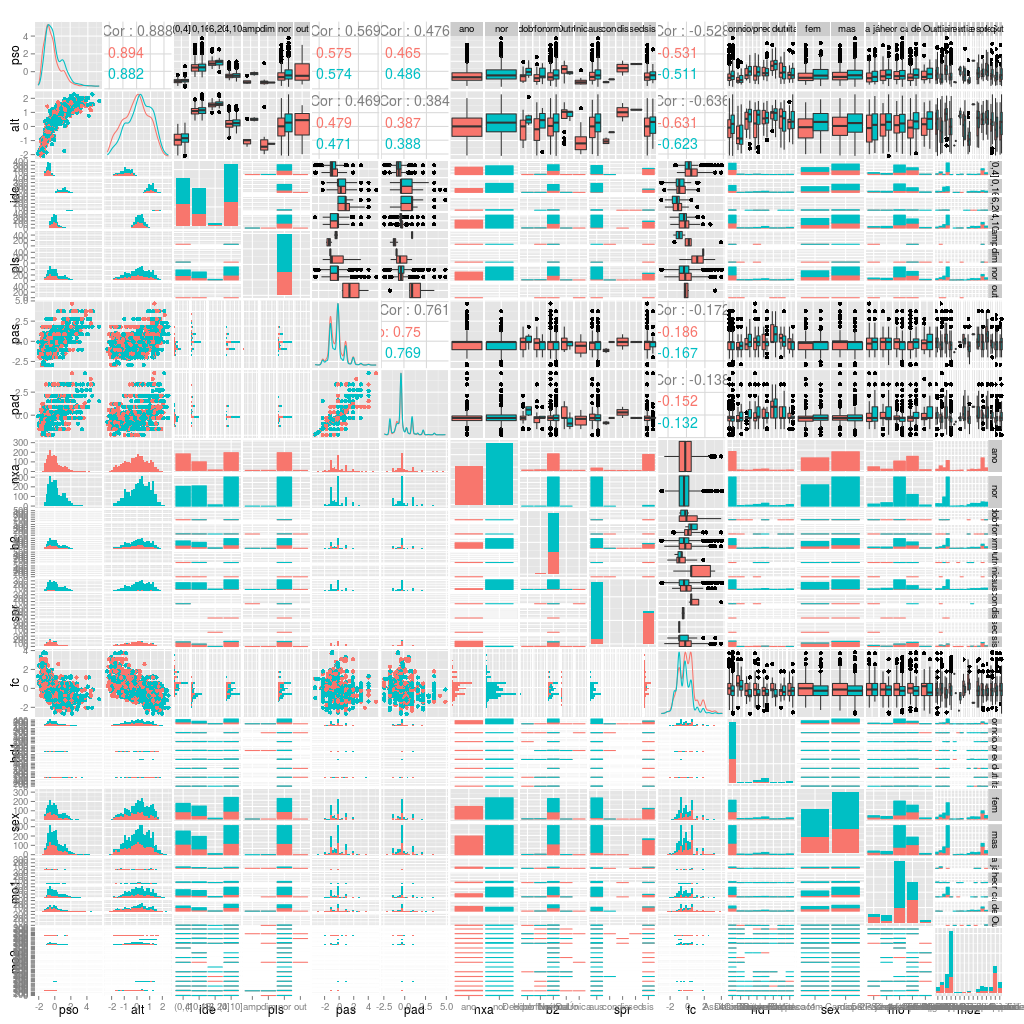
\includegraphics[scale=0.5]{img/final_scattermatrix.png}
  \caption{\textit{Scatter Matrix} dos dados preprocessados}
  \label{fig:finalsm}
\end{figure*}

\begin{table*}[!htbp] \centering 
  \caption{Sumário dos atributos numéricos preprocessados}
  \label{tab:nuf} 
  \begin{tabular}{@{\extracolsep{5pt}}lccccc} 
    \\[-1.8ex]\hline 
    \hline \\[-1.8ex] 
    Estatística & {\tt pso} & {\tt alt} & {\tt pas} & {\tt pad} & {\tt fc} \\ 
    \hline \\[-1.8ex] 
    Média & 0.1 & 0.1 & $-$0.2 & $-$0.2 & $-$0.1 \\ 
    Desvio Padrão & 1.0 & 0.9 & 0.9 & 0.9 & 0.9 \\ 
    Mínimo & $-$1.7 & $-$2.2 & $-$2.9 & $-$2.1 & $-$2.7 \\ 
    Máximo & 5.3 & 2.6 & 5.6 & 4.5 & 3.8 \\ 
    \hline \\[-1.8ex] 
  \end{tabular} 
\end{table*}


% ----------------------------------------
% -                                      -
% ----------------------------------------

\section{Análise final}
\label{sec:afn}

A análise final será dividida em 3 partes com objetivos diferentes. A
primeira irá olhar para cada par de atributos e procurará relações
entre eles. Com este conhecimento, fazemos uma análise multivariável
que pretenderá perceber a relação entre conjuntos de variáveis, com o
objetivo de escolher os melhores atributos para prever {\tt
  nxa}. Finalmente, aplicaremos os resultados obtidos a algoritmos de
previsão e mediremos o seu comportamento.

% ----------------------------------------

\subsection{Análise bivariável}
Esta análise incidirá principalmente sobre 3 métricas: correlação
linear (de Pearson), regressão linear, e distância de correlação. O
objetivo da última métrica é o de encontrar relações não lineares
entre atributos numéricos. É importante notar que estas métricas só se
aplicam a dados numéricos e por isso toda esta análise apenas incidirá
sobre os dados numéricos que possuímos.

É possível observar as correlações lineares na matriz de correlações
lineares representada na Tabela~\ref{tab:cmt}. Com pequenas exceções,
todos os dados estão relativamente bem correlacionados, com alguns
picos para o par {\tt pso} e {\tt alt} e para o par {\tt pas} e {\tt
  pad}, pois são atributos análogos.

Para estudar os dados usando regressões lineares, foram feitas
regressões lineares entre cada par e estudado o erro quadrado da
previsão usando a regressão (de forma semelhante ao que foi feito na
Secção~\ref{sec:pre}). Este erro está representado em forma de matriz
na Tabela~\ref{tab:rmt}. É possível observar valores baixos de erro para
vários pares de atributos. Isto pode ser observado graficamente
através de \textit{scatter plots} onde são traçadas as retas de
regressão. Para o par {\tt pso} e {\tt alt} a Figura~\ref{fig:reg1}
mostra o seu gráfico de regressão. Para o par {\tt pas} e {\tt pad} a
Figura~\ref{fig:reg2} mostra o seu gráfico de regressão. Finalmente,
para o par {\tt pad} e {\tt fc} a Figura~\ref{fig:reg3} mostra o seu
gráfico de regressão. No primeiro caso é possível observar que existe
uma relação entre os dois atributos, mas não é necessariamente
linear. No segundo caso há uma relação claramente linear. No último
caso existem indícios de alguma relação, embora não seja tão forte.

A última métrica, a distância de correlação, está sumarizada na
Tabela~\ref{tab:dmt}. Os resultados não revelam muita diferença para o
caso linear, de onde se conclui que as relações dos dados são
aproximadamente lineares.

\begin{figure}[H]
  \centering
  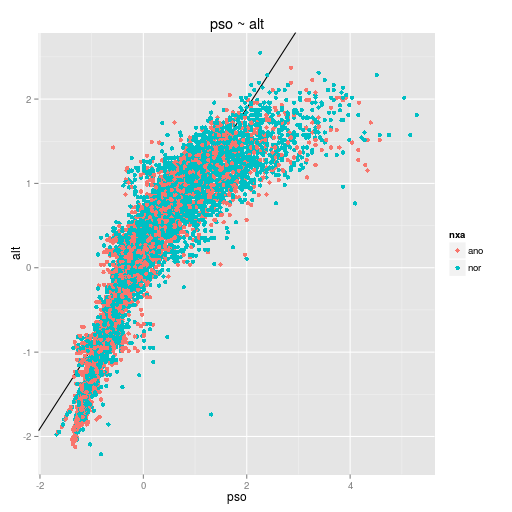
\includegraphics[scale=0.4]{img/reg_pso_alt.png}
  \caption{Regressão entre {\tt pso} e {\tt alt}}
  \label{fig:reg1}
\end{figure}

\begin{figure}[H]
  \centering
  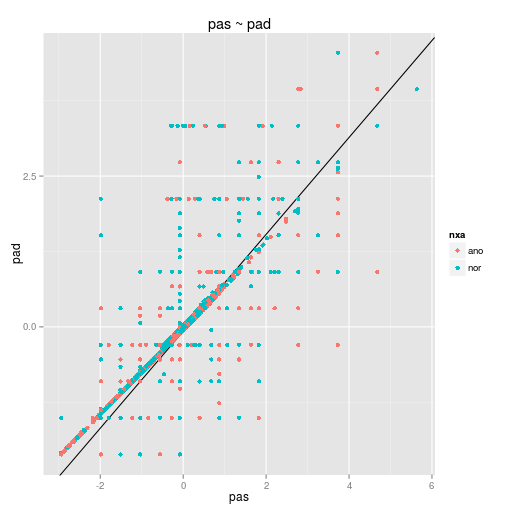
\includegraphics[scale=0.4]{img/reg_pas_pad.png}
  \caption{Regressão entre {\tt pas} e {\tt pad}}
  \label{fig:reg2}
\end{figure}

\begin{figure}[H]
  \centering
  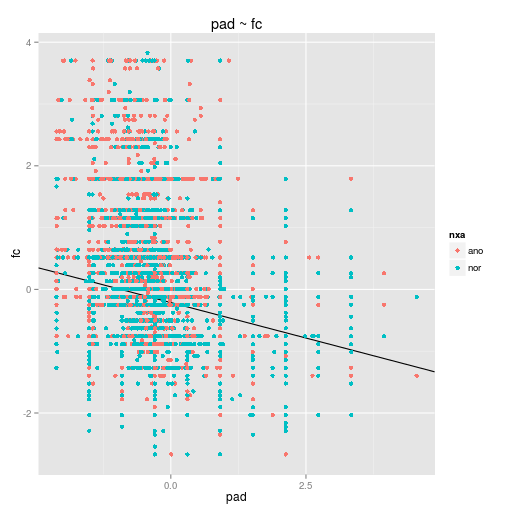
\includegraphics[scale=0.4]{img/reg_pad_fc.png}
  \caption{Regressão entre {\tt pad} e {\tt fc}}
  \label{fig:reg3}
\end{figure}

\begin{table*}[!ht] \centering 
  \caption{Matriz de correlações lineares}
  \label{tab:cmt}
  \begin{tabular}{@{\extracolsep{5pt}} cccccc} 
    \\[-1.8ex]\hline 
    \hline \\[-1.8ex] 
    & {\tt pso} & {\tt alt} & {\tt pas} & {\tt pad} & {\tt fc} \\ 
    \hline \\[-1.8ex] 
    {\tt pso} & $1.000$ & $0.896$ & $0.616$ & $0.505$ & $-0.542$ \\ 
    {\tt alt} & $0.896$ & $1.000$ & $0.532$ & $0.427$ & $-0.650$ \\ 
    {\tt pas} & $0.616$ & $0.532$ & $1.000$ & $0.758$ & $-0.311$ \\ 
    {\tt pad} & $0.505$ & $0.427$ & $0.758$ & $1.000$ & $-0.238$ \\ 
    {\tt fc}  & $-0.542$ & $-0.650$ & $-0.311$ & $-0.238$ & $1.000$ \\ 
    \hline \\[-1.8ex] 
  \end{tabular} 
\end{table*}

\begin{table*}[!htbp] \centering 
  \caption{Matriz de regressões lineares}
  \label{tab:rmt}
  \begin{tabular}{@{\extracolsep{5pt}} cccccc} 
    \\[-1.8ex]\hline 
    \hline \\[-1.8ex]
    & {\tt pso} & {\tt alt} & {\tt pas} & {\tt pad} & {\tt fc} \\
    \hline \\[-1.8ex] 
    {\tt pso} & $0.000$ & $0.000$ & $0.180$ & $0.180$ & $0.070$ \\ 
    {\tt alt} & $0.000$ & $0.000$ & $0.230$ & $0.240$ & $0.070$ \\ 
    {\tt pas} & $0.180$ & $0.230$ & $0.000$ & $0.000$ & $0.070$ \\ 
    {\tt pad} & $0.180$ & $0.240$ & $0.000$ & $0.000$ & $0.050$ \\ 
    {\tt fc}  & $0.070$ & $0.070$ & $0.070$ & $0.050$ & $0.000$ \\ 
    \hline \\[-1.8ex] 
  \end{tabular} 
\end{table*} 

\begin{table*}[!htbp] \centering 
  \caption{Matriz de distâncias de correlação}
  \label{tab:dmt}
  \begin{tabular}{@{\extracolsep{5pt}} cccccc}
    \\[-1.8ex]\hline 
    \hline \\[-1.8ex]
    & {\tt pso} & {\tt alt} & {\tt pas} & {\tt pad} & {\tt fc} \\
    \hline \\[-1.8ex] 
    {\tt pso} & $1.000$ & $0.916$ & $0.581$ & $0.456$ & $0.560$ \\
    {\tt alt} & $0.922$ & $1.000$ & $0.504$ & $0.433$ & $0.619$ \\
    {\tt pas} & $0.583$ & $0.511$ & $1.000$ & $0.719$ & $0.303$ \\
    {\tt pad} & $0.486$ & $0.438$ & $0.721$ & $1.000$ & $0.246$ \\
    {\tt fc}  & $0.554$ & $0.623$ & $0.335$ & $0.245$ & $1.000$ \\
    \hline \\[-1.8ex] 
  \end{tabular} 
\end{table*}


% ----------------------------------------

\subsection{Análise multivariável}
Parte desta análise já foi efetuada na Secção~\ref{sec:pre} quando se
fez preenchimento dos dados (nas regressões multivariável), mas
complementamos essa análise com métodos diferentes para conclusões
diferentes.

Para perceber a relação entre as variáveis foi efetuado uma análise
componentes principais. Aplicamos o algoritmo de $PCA$ para os
atributos numéricos dos dados. Os desvios padrão obtidos para as 5
componentes estão descritos na Figura~\ref{fig:ampca}.

Visto que as duas componentes contêm aproximadamente $70\%$ da
variância dos atributos, decidimos manter apenas as duas primeiras
componentes. Com isto afirmamos que a maior parte da informação
contida nos 5 atributos numéricos dos dados é comprimível até 2
atributos. Este resultado é espectável visto que há pelo menos dois
pares de atributos muito correlacionados.

Munidos dos dados comprimidos, começamos por fazer uma análise de
\textit{clustering}. Escolhemos um \textit{clustering} hierárquico
usando o método de \textit{Ward} por ser fácil de interpretar e por
gerar grupos densos e esféricos. O resultado obtido está representado
na Figura~\ref{fig:ampcahs}.

\begin{figure}[H]
  \centering
  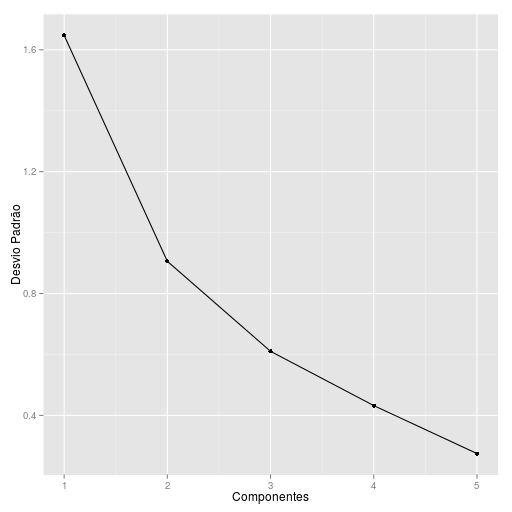
\includegraphics[scale=0.4]{img/amv_pcasd.png}
  \caption{Desvios padrão para as componentes do $PCA$}
  \label{fig:ampca}
\end{figure}

Pela observação do resultado é possível delinear alguns
\textit{clusters} bem definidos (com distância entre si relativamente
baixa). Representámos estes por retângulos a vermelho na
Figura~\ref{fig:ampcahs}. A razão para termos escolhido 7
\textit{clusters} é puramente heurística e baseada na observação da
figura. Este resultado será útil para complementar uma análise que
faremos mais à frente.

\begin{figure}[H]
  \centering
  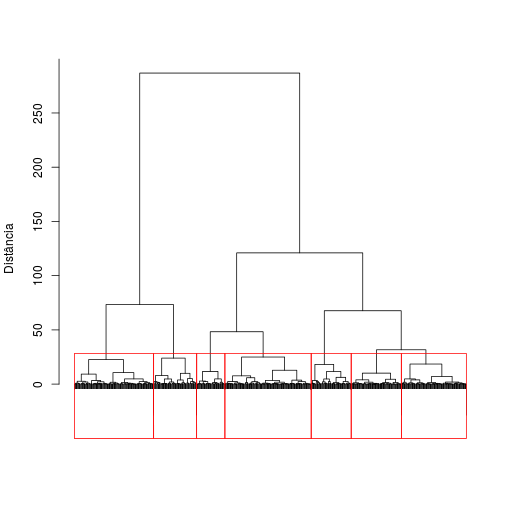
\includegraphics[scale=0.4]{img/amv_pcahc.png}
  \caption{\textit{Clustering} hierárquico para os dados comprimidos}
  \label{fig:ampcahs}
\end{figure}

Um outro dado importante que pode ser extraído dos dados comprimidos é
a sua relação com o atributo a prever, o {\tt nxa}. Sendo assim
representamos num \textit{scatter plot} a sua distribuição e colorimos
os pontos com a devida classe de {\tt nxa}. O resultado pode ser
observado na Figura~\ref{fig:ampcast}.

\begin{figure}[H]
  \centering
  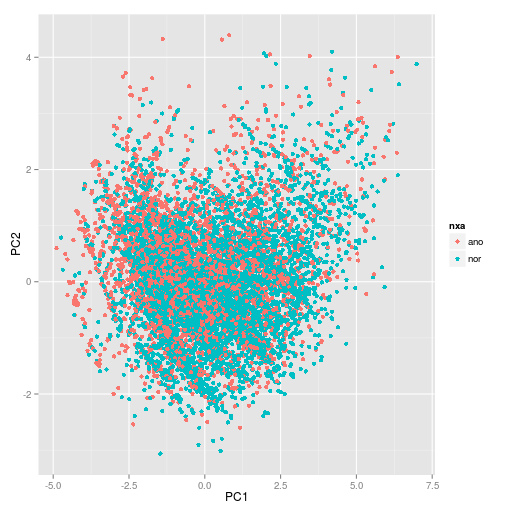
\includegraphics[scale=0.4]{img/amv_pcast.png}
  \caption{\textit{Scatter plot} para as componentes do $PCA$ em relação a {\tt nxa}}
  \label{fig:ampcast}
\end{figure}

É possível observar que a distribuição dos {\tt nxa} não é bem
dividida pelas componentes dos dados. Apesar de existir uma ligeira
tendência para os pacientes com valor de {\tt PC1} baixo possuírem uma
anomalia, não é fácil de prever a classe de {\tt nxa} segundo as duas
componentes principais. Assim, concluímos que os atributos numéricos
dos dados não têm um bom poder de previsão de {\tt nxa}.

Continuámos a análise aplicando algoritmos de \textit{clustering} de
partição nos dados originais (não usaremos mais os dados obtidos pelo
$PCA$ no resto do relatório). Usámos o algoritmo de \textit{Lloyd} com
3 \textit{random restarts} por ser um dos mais comuns e por ser fácil
de interpretar. Para determinar o valor de $k$ a usar corremos o
algoritmo com diferentes valores e representámos o erro que cada um
obteve. Os resultados podem ser observados na
Figura~\ref{fig:amkmdis}.

\begin{figure}[H]
  \centering
  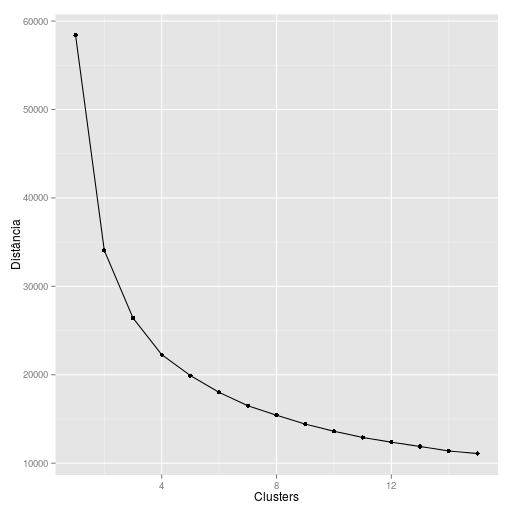
\includegraphics[scale=0.4]{img/amv_kmdis.png}
  \caption{Erro associado a cada \textit{cluster} para diferentes $k$s}
  \label{fig:amkmdis}
\end{figure}

Usando a heurística do ``cotovelo'' assim como os resultados obtidos
anteriormente para o $PCA$, escolhemos 7 como o número de
\textit{clusters} para efetuar a análise.

Tendo gerado os \textit{clusters}, representamos os dados em pares de
\textit{scatter plots} e colorimos cada ponto com uma cor
representativa do \textit{cluster}. O resultado encontra-se na
Figura~\ref{fig:amksm}.

\begin{figure*}[!ht]
  \centering
  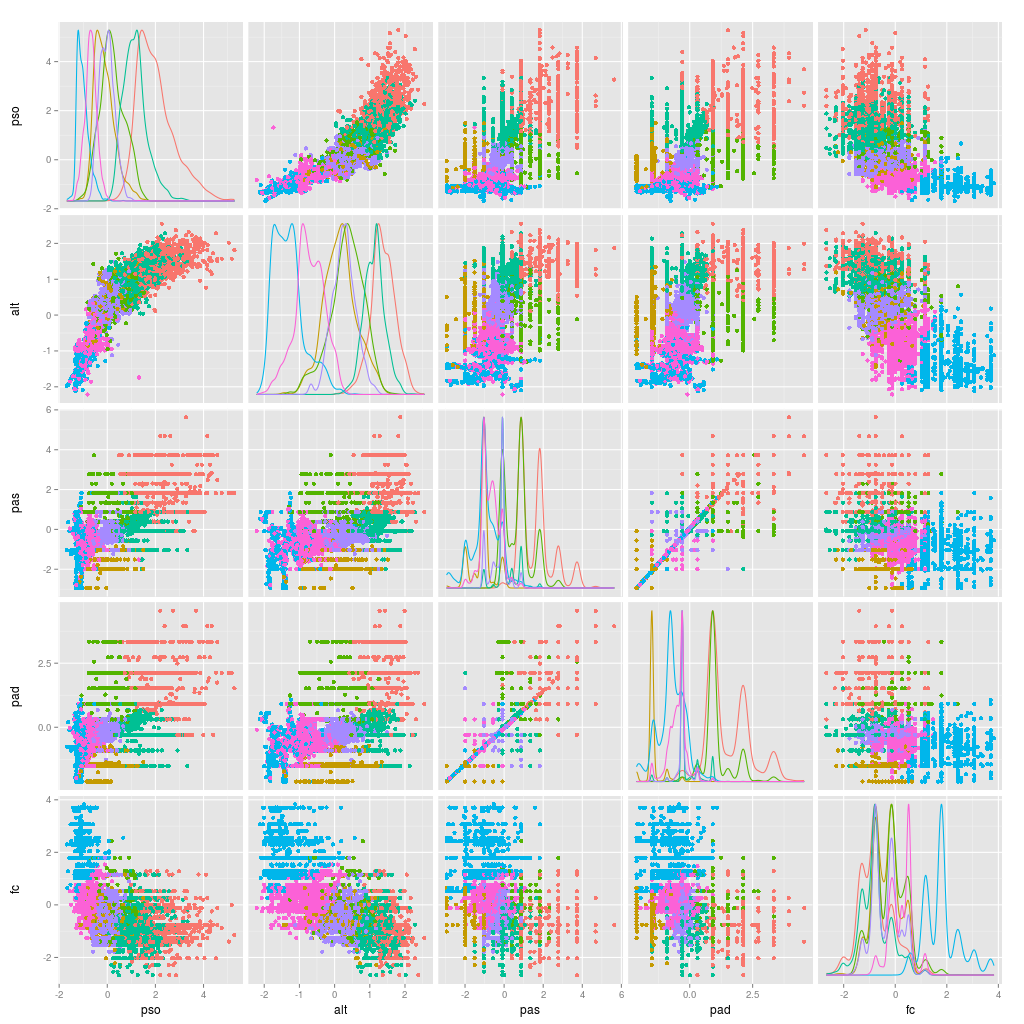
\includegraphics[scale=0.5]{img/amv_kmsm.png}
  \caption{Pares de \textit{scatter plots} com \textit{clusters}}
  \label{fig:amksm}
\end{figure*}

Observando a distribuição dos atributos em relação a cada
\textit{cluster}, é possível identificar aproximações a distribuições
normais bem definidas. Além desta análise mais simples, seria possível
uma análise mais profunda usando métodos como \textit{association rule
  mining}, para determinar tendências entre os dados a partir dos
\textit{clusters}. Por exemplo, é possível identificar o
\textit{cluster} vermelho na Figura~\ref{fig:amksm} por pacientes com
       {\tt pso}, {\tt alt}, {\tt pas} e {\tt pad} elevados, mas {\tt
         fc} baixo, o que é consistente com as correlações encontradas
       na subsecção anterior e com os intervalos normais associados a
       indivíduos de idades entre os 16 e 20 anos. Embora haja muito
       espaço para mais análise neste sentido, por brevidade será
       omitida.

% ----------------------------------------

\subsection{Análise de previsão}

\lipsum[4]

% ----------------------------------------

\subsubsection{Comparação de métodos}

\lipsum[5]

% ----------------------------------------
% -                                      -
% ----------------------------------------

\section{Conclusão e discussão}
\label{sec:cnd}

\lipsum[4]
\cite{boser1992training}

\small
\begin{spacing}{0.92}
\bibliographystyle{IEEEtran}
\bibliography{IEEEabrv,report}
\end{spacing}

\end{document}


